\documentclass[12pt]{beamer}


\usetheme[progressbar=frametitle]{metropolis}
\usepackage{appendixnumberbeamer}

\usepackage{booktabs}
\usepackage[scale=2]{ccicons}

%\usepackage{pgfplots}
%\usepgfplotslibrary{dateplot}

\usepackage{xspace}
\newcommand{\themename}{\textbf{\textsc{metropolis}}\xspace}

%\setbeamertemplate{footline} % To remove the footer line in all slides uncomment this line
%\setbeamertemplate{footline}[page number] % To replace the footer line in all slides with a simple slide count uncomment this line

%\setbeamertemplate{navigation symbols}{} % To remove the navigation symbols from the bottom of all slides uncomment this line


\usepackage{graphicx} % Allows including images
\usepackage{grffile}
\usepackage{amsmath}
\usepackage{adjustbox} 
% have to have Mozilla's=Fira Sans} font and XeTeX installed to use full typography.

%----------------------------------------------------------------------------------------
%	TITLE PAGE
%----------------------------------------------------------------------------------------

\title{Collective Action or Exchange?: Framing International Cooperation in Alliance Politics}
\date{November 12, 2020}
\author{Joshua Alley}
\institute{University of Virginia}


\begin{document}

 \maketitle


%----------------------------------------------------------------------------------------
%	PRESENTATION SLIDES
%----------------------------------------------------------------------------------------

%------------------------------------------------
% Here's my question. 
 \begin{frame}[standout]

How do elite frames of allied military spending affect public support for cooperation in alliances? 

 \end{frame}
 

%------------------------------------------------

\begin{frame}{Why Should You Care?}

\begin{figure}[htbp]
		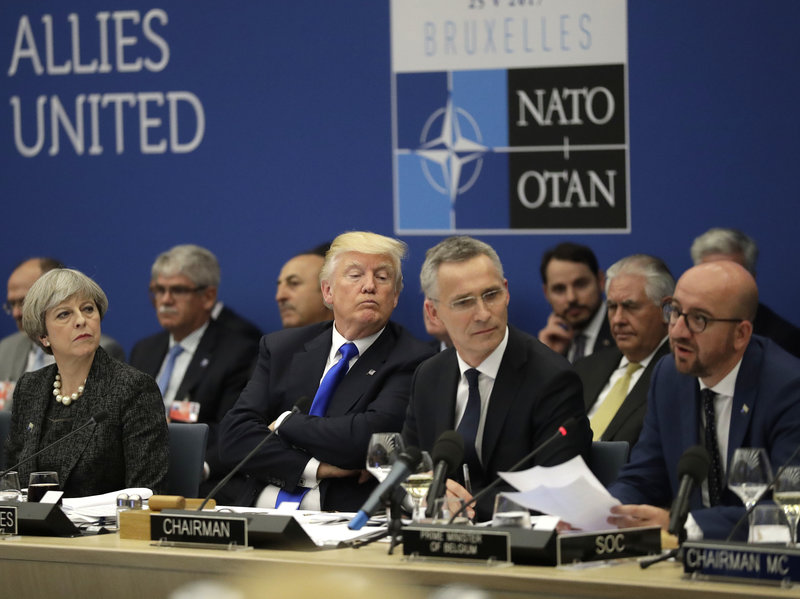
\includegraphics[width=0.95\textwidth]{trump-nato.jpg}
	\label{fig:trump-nato}
\end{figure}


\end{frame}


%------------------------------------------------

\begin{frame}{Outline}

\pause
\begin{enumerate}
\item Argument: Frames and alliance member size. 
\pause
\item Survey Experiment Design. 
\pause
\item Pretest Results from the US and Germany.  
\end{enumerate}


\end{frame}
 

%------------------------------------------------

\section{Argument} 

%-----------------------------------------------

\begin{frame}{Two Frames of International Cooperation}

Can explain the causes and consequences of cooperation with:

\pause 
\begin{enumerate} 
\item \textbf{Collective Action}: Cooperate by contributing to some common/public good. 
\pause 
\item \textbf{Exchange}: Cooperate by trading different goods. 
\end{enumerate}


\end{frame} 

%-----------------------------------------------

\begin{frame}{Framing Spending by Alliance Members}

The two frames can explain differences in military spending between small and large alliance members. 

\pause 
\begin{enumerate} 
\item \textbf{Collective Action}: Free-riding and disproportionate contributions. 
\pause 
\item \textbf{Exchange}: Trading different foreign policy goods- security for influence. 
\end{enumerate}


\end{frame} 

%-----------------------------------------------

\begin{frame}[standout]

These frames have opposite effects on attitudes towards alliances in leading and junior states. 

\end{frame} 

%-----------------------------------------------

\begin{frame}{Leading States}

Given disproportionate defense spending by the alliance leader:  
\pause 
\begin{enumerate} 
\item \textbf{Collective Action Framing}: Decreases support for cooperation: conditional cooperation and exploitation aversion. 
\pause 
\item \textbf{Exchange Framing}: Increases support for cooperation: reciprocity. 
\end{enumerate}


\end{frame} 

%-----------------------------------------------

\begin{frame}{Junior States}

Given disproportionate defense spending by the alliance leader: 
\pause 
\begin{enumerate} 
\item \textbf{Collective Action Framing}: Increases support for cooperation: conditional cooperation and perceptions of benevolent leadership. 
\pause 
\item \textbf{Exchange Framing}: Decreases support for cooperation: reduces leader legitimacy. 
\end{enumerate}


\end{frame} 

%-----------------------------------------------

\begin{frame}{Summary of Predictions}

\resizebox{.95\textwidth}{!}{
\begin{tabular}{|l|c|c|}

\hline
            & Large   & Small \\ \hline
Collective & Decrease    & Increase \\ \hline
Exchange   & Increase   & Decrease \\
\hline
\end{tabular}
}

\end{frame} 




%------------------------------------------------

\section{Experimental Design} 

%-----------------------------------------------

\begin{frame}{Sample}

Two studies examining attitudes towards NATO in the United States and Germany. 210 respondents in each study. Randomly assign neutral, collective action or exchange vignette about NATO and military spending. 

\pause 
\begin{enumerate} 
\item Favorability towards NATO. 
\pause 
\item Support for withdrawal (US) or higher defense spending (Germany).  
\pause
\item Support for military intervention. 
\end{enumerate}


\end{frame} 

%-----------------------------------------------

\begin{frame}{Vignettes}


\begin{enumerate}

\item \textbf{Neutral}: (Your Country) has an important role in the North Atlantic Treaty Organization (NATO). NATO is a military alliance where members promise to support one another in war. According to an expert at the Council on Foreign Relations, a non-partisan think tank, some NATO members spend a smaller share of their resources on the military than the United States. 
\pause
\item \textbf{Collective Action}: adds \textit{because other states make limited contributions to collective security, and count on the United States to carry the load.} 
\pause
\item \textbf{Exchange}: adds \textit{because they support US priorities and interests in international politics in exchange for protection by the United States.}
 
\end{enumerate} 

\end{frame} 


%-----------------------------------------------

\begin{frame}{Response Questions}


\begin{enumerate}

\item \textbf{Favorability}: 1-5 scale from Very Unfavorable to Very Favorable.  
\pause 
\item \textbf{Policy Change}: Yes/No on withdrawal (US) and military spending (Germany). 
\pause 
\item \textbf{Intervention}: Yes/No. 
 
\end{enumerate} 

\end{frame} 



%------------------------------------------------

\section{Pretest Results} 

%-----------------------------------------------


\begin{frame}{United States: Raw Data}

\begin{figure}[htbp]
	\centering
		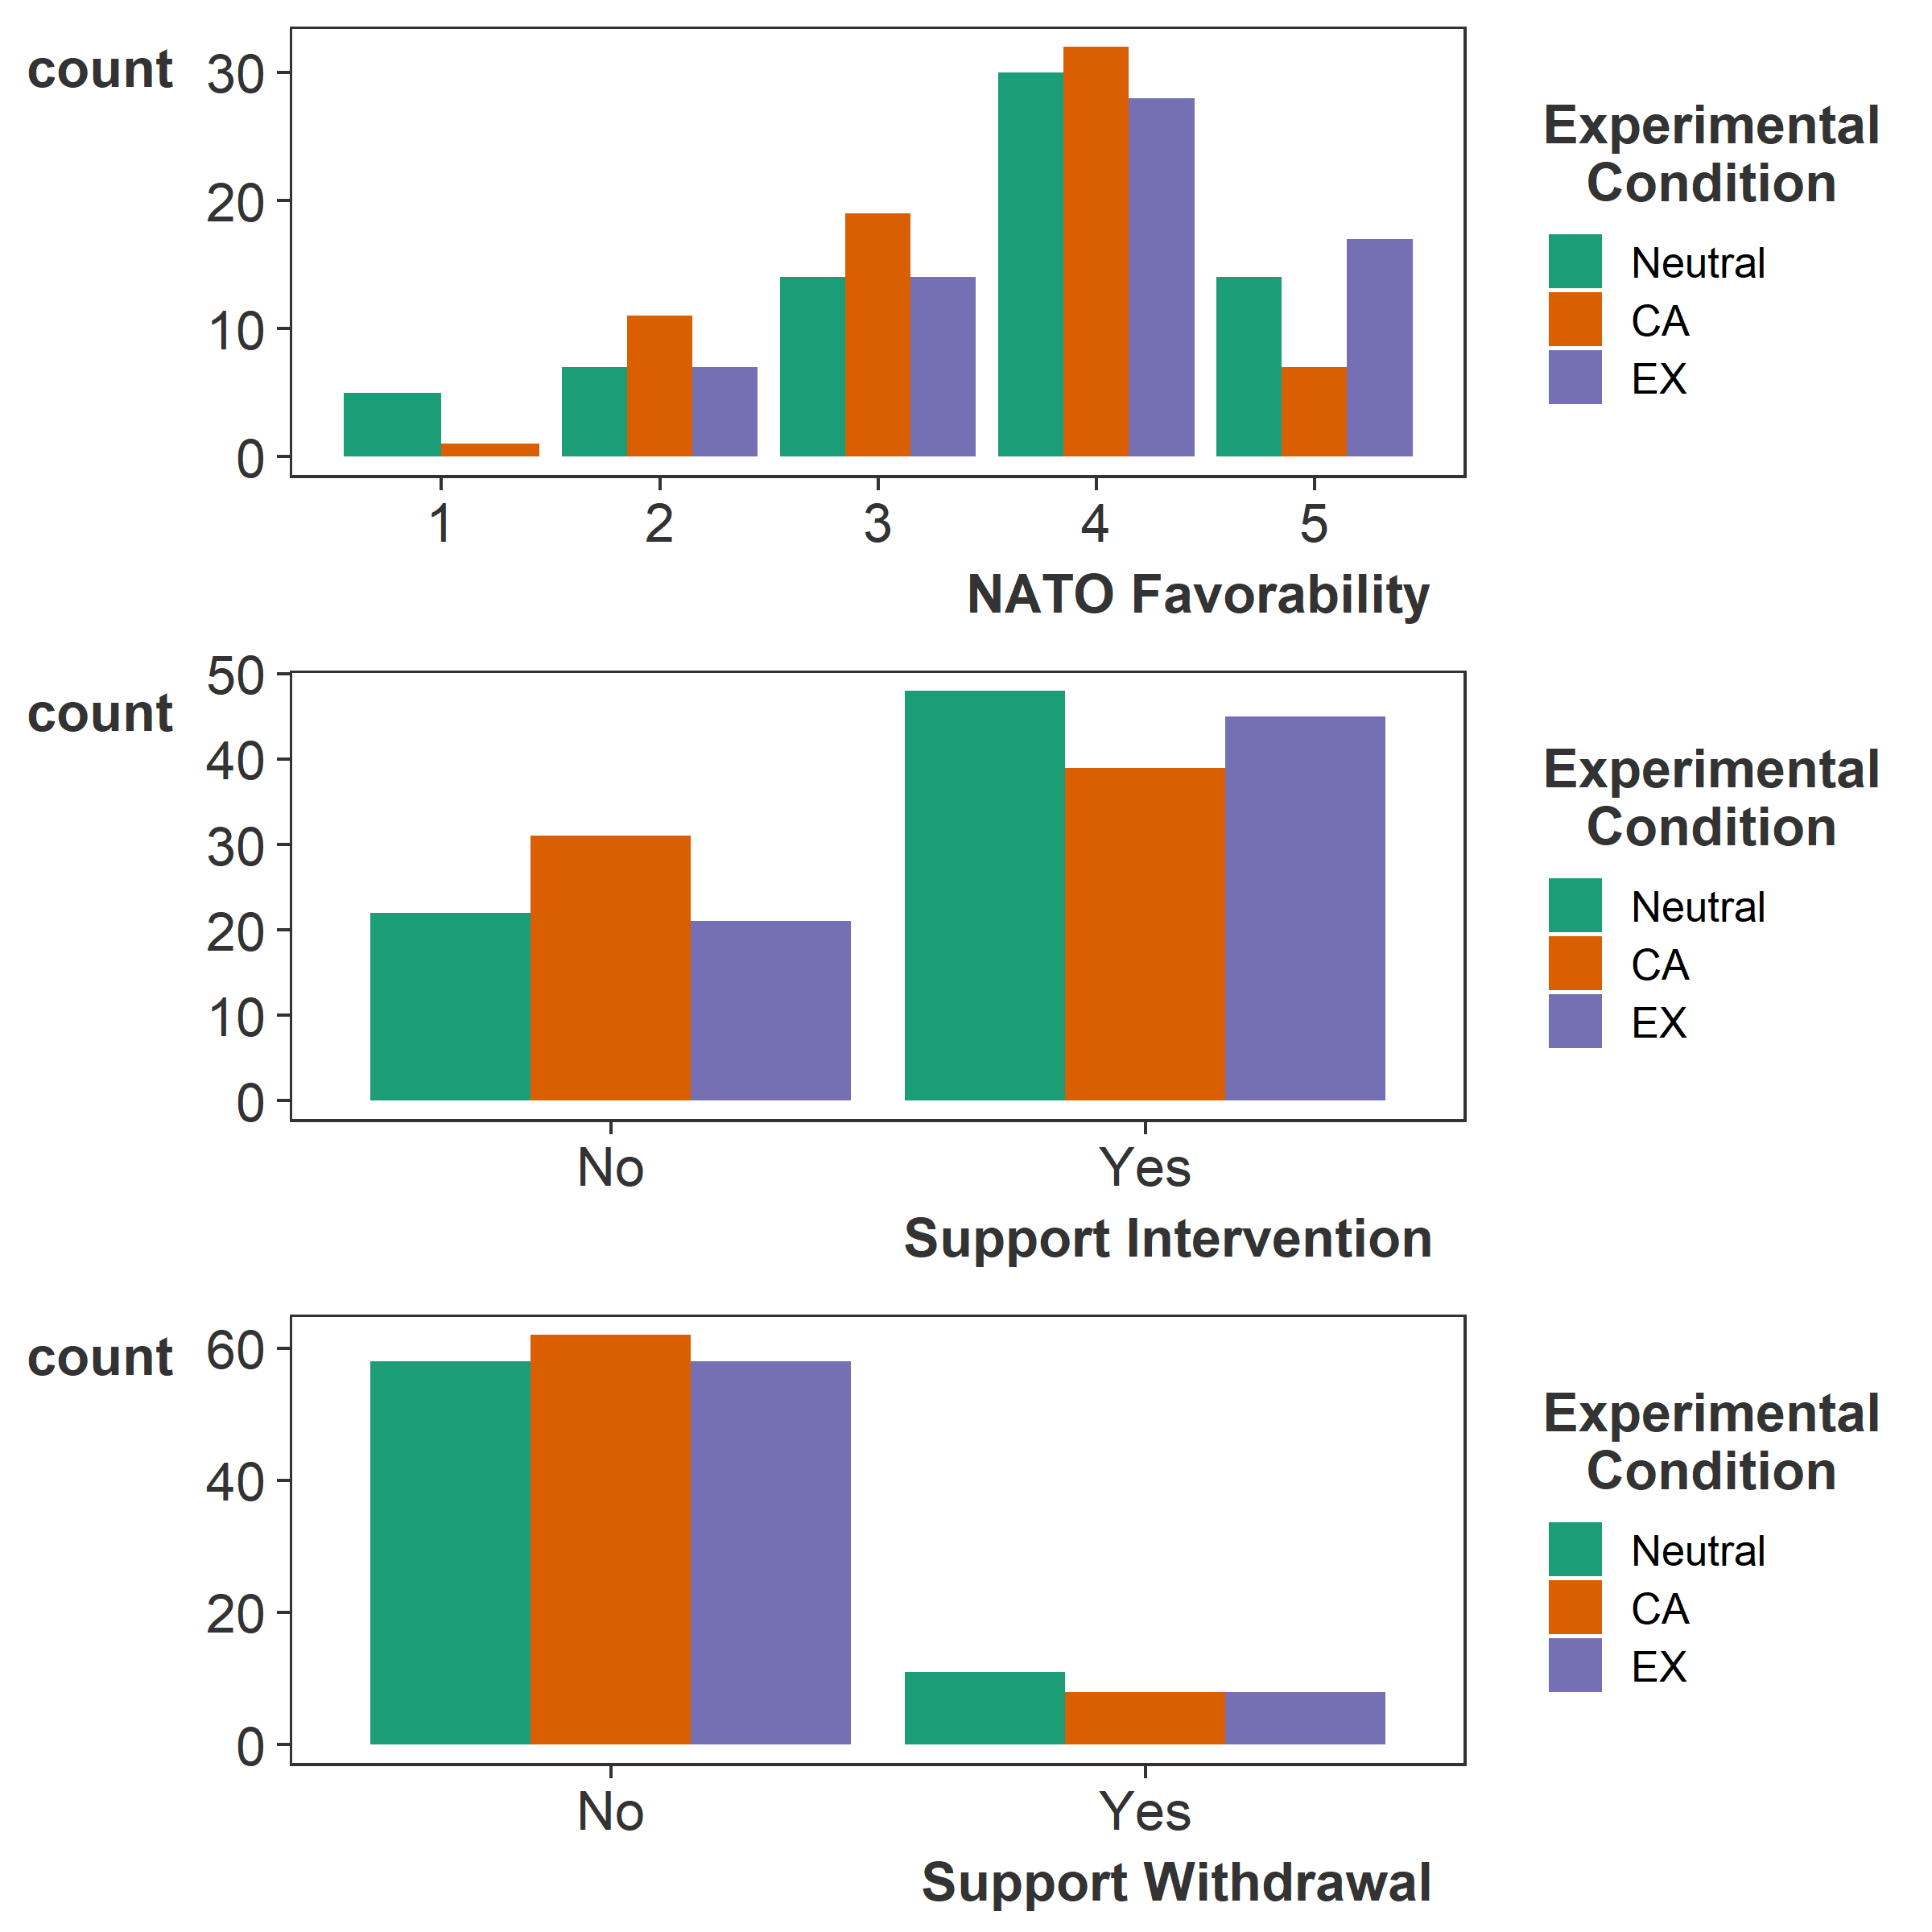
\includegraphics[height=.95\textheight]{raw-us-pres.png}
\end{figure}


\end{frame}

%-----------------------------------------------

\begin{frame}{United States: Treatment Effects}

% mention regressions
\pause 

\begin{figure}[htbp]
	\centering
		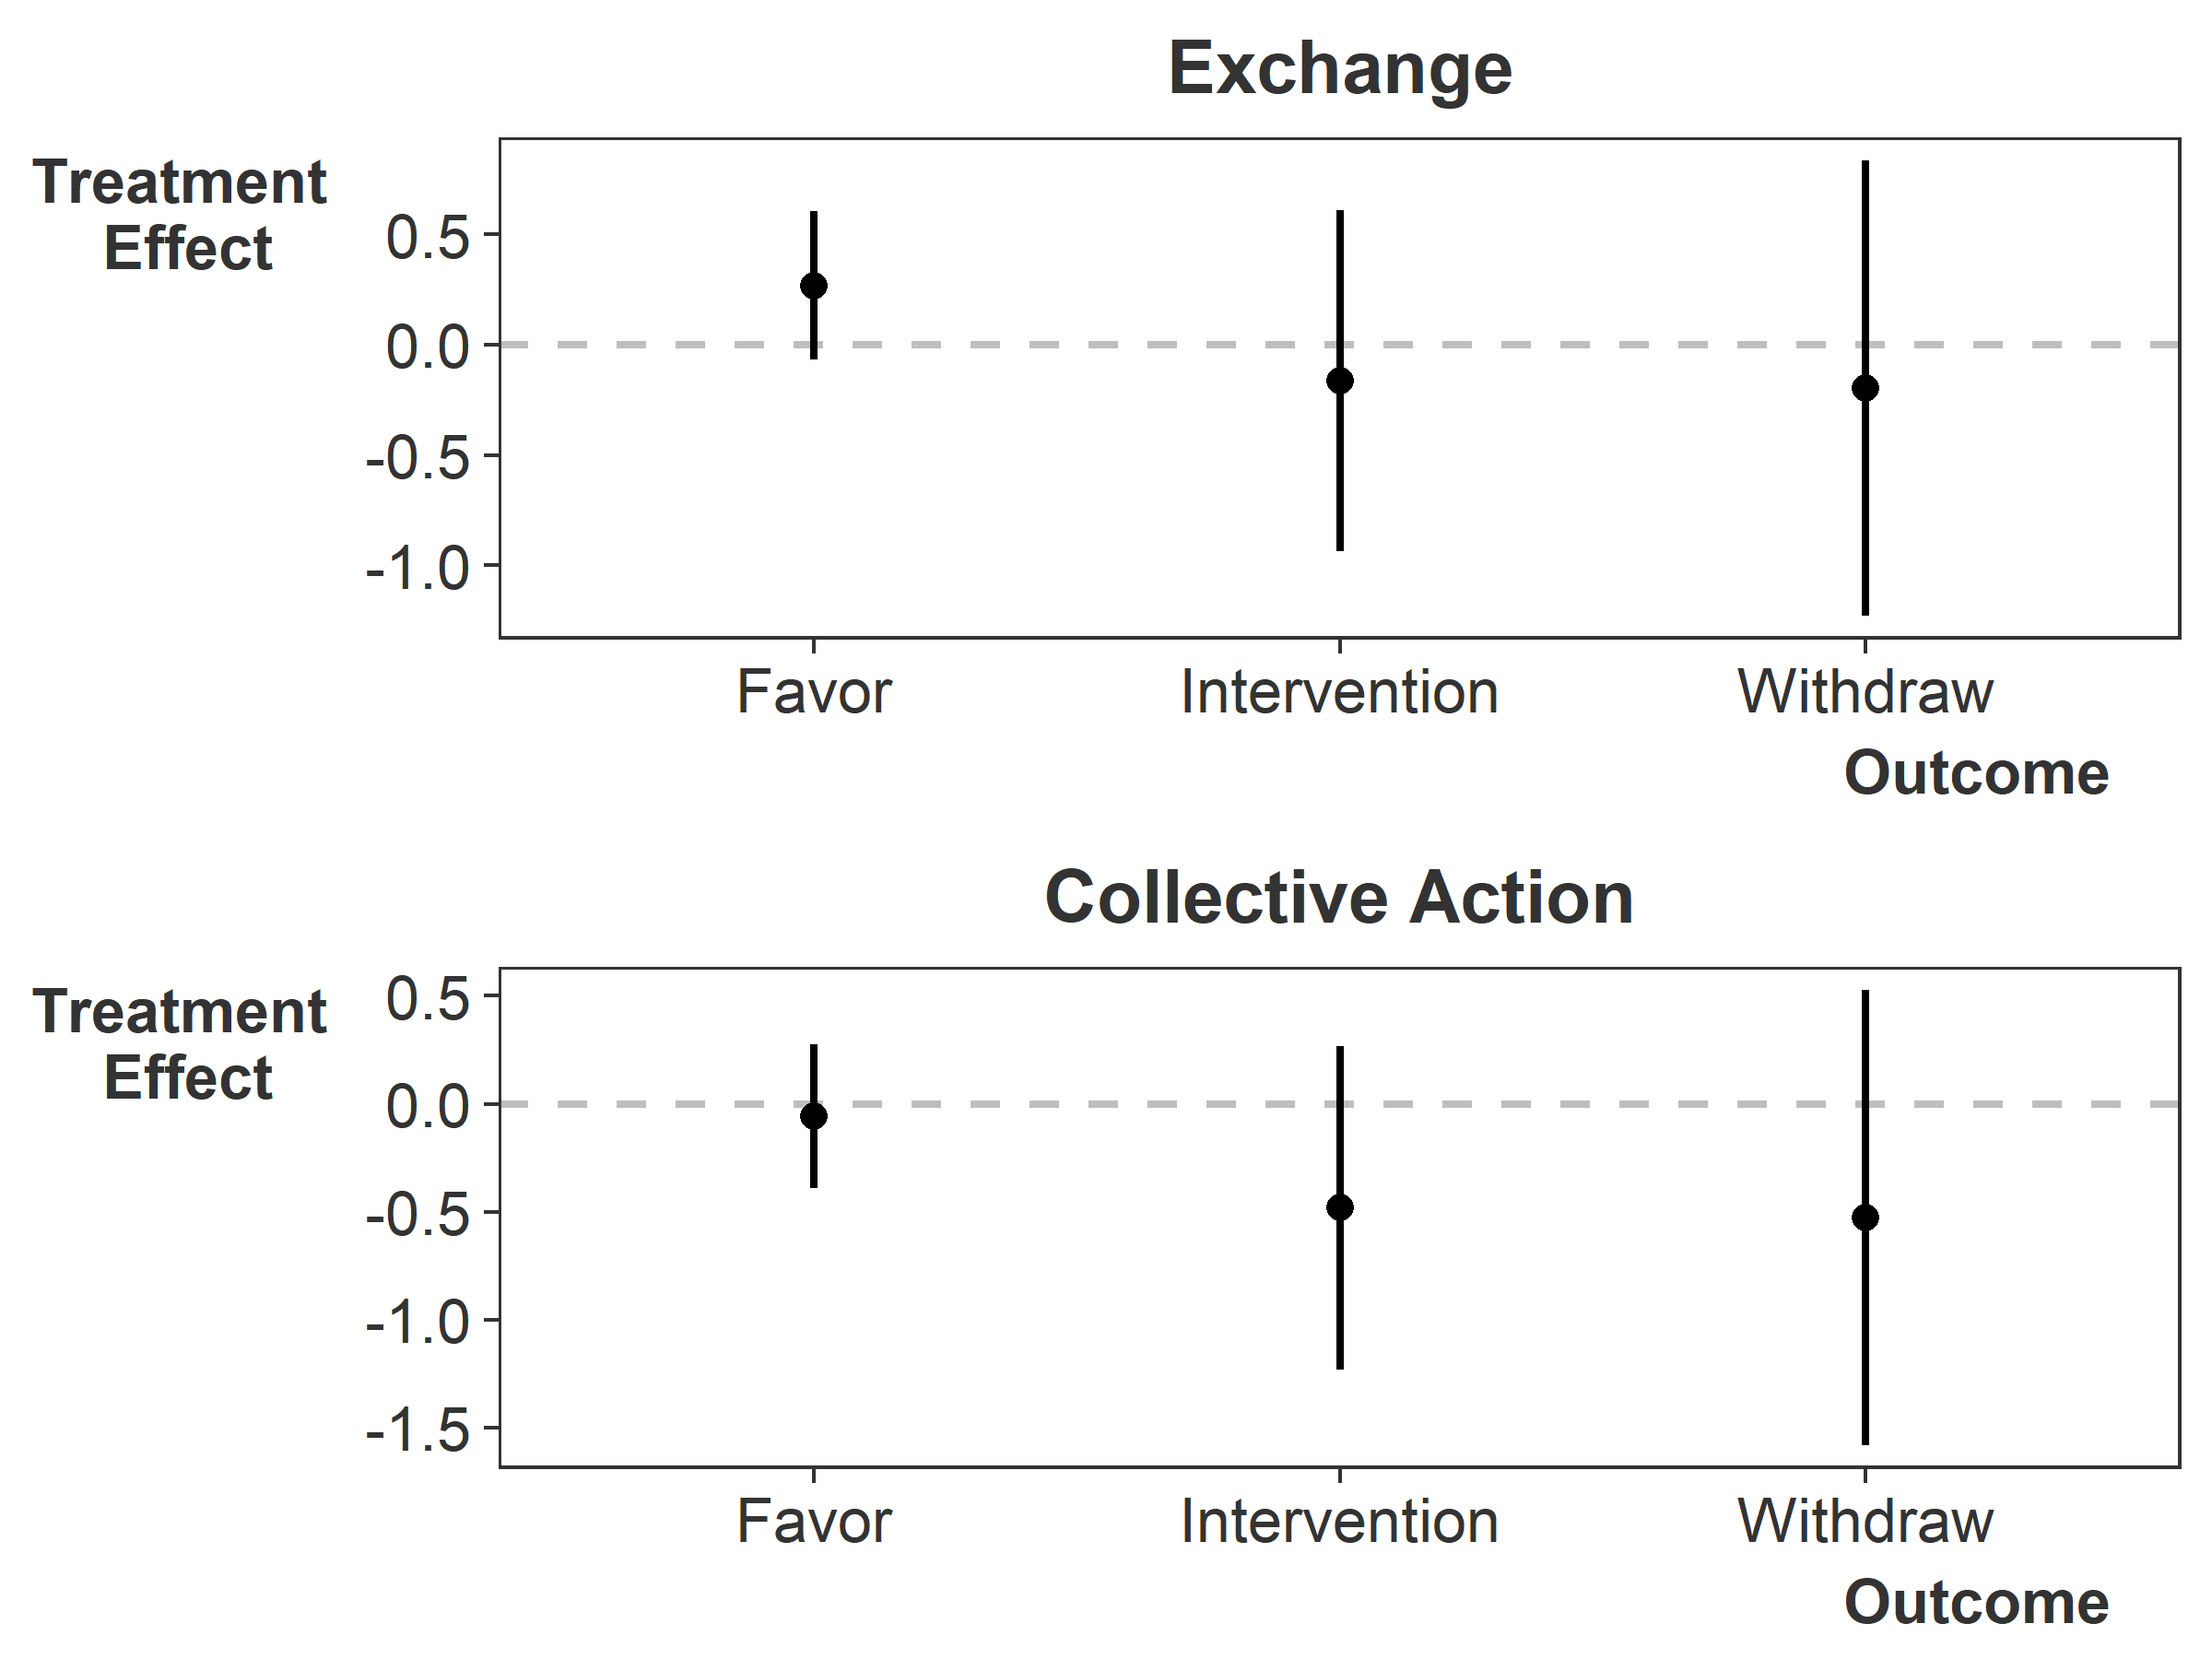
\includegraphics[width=0.95\textwidth]{us-te-pres.png}
\end{figure}


\end{frame}

%-----------------------------------------------


\begin{frame}{Germany: Raw Data}

\begin{figure}[htbp]
	\centering
		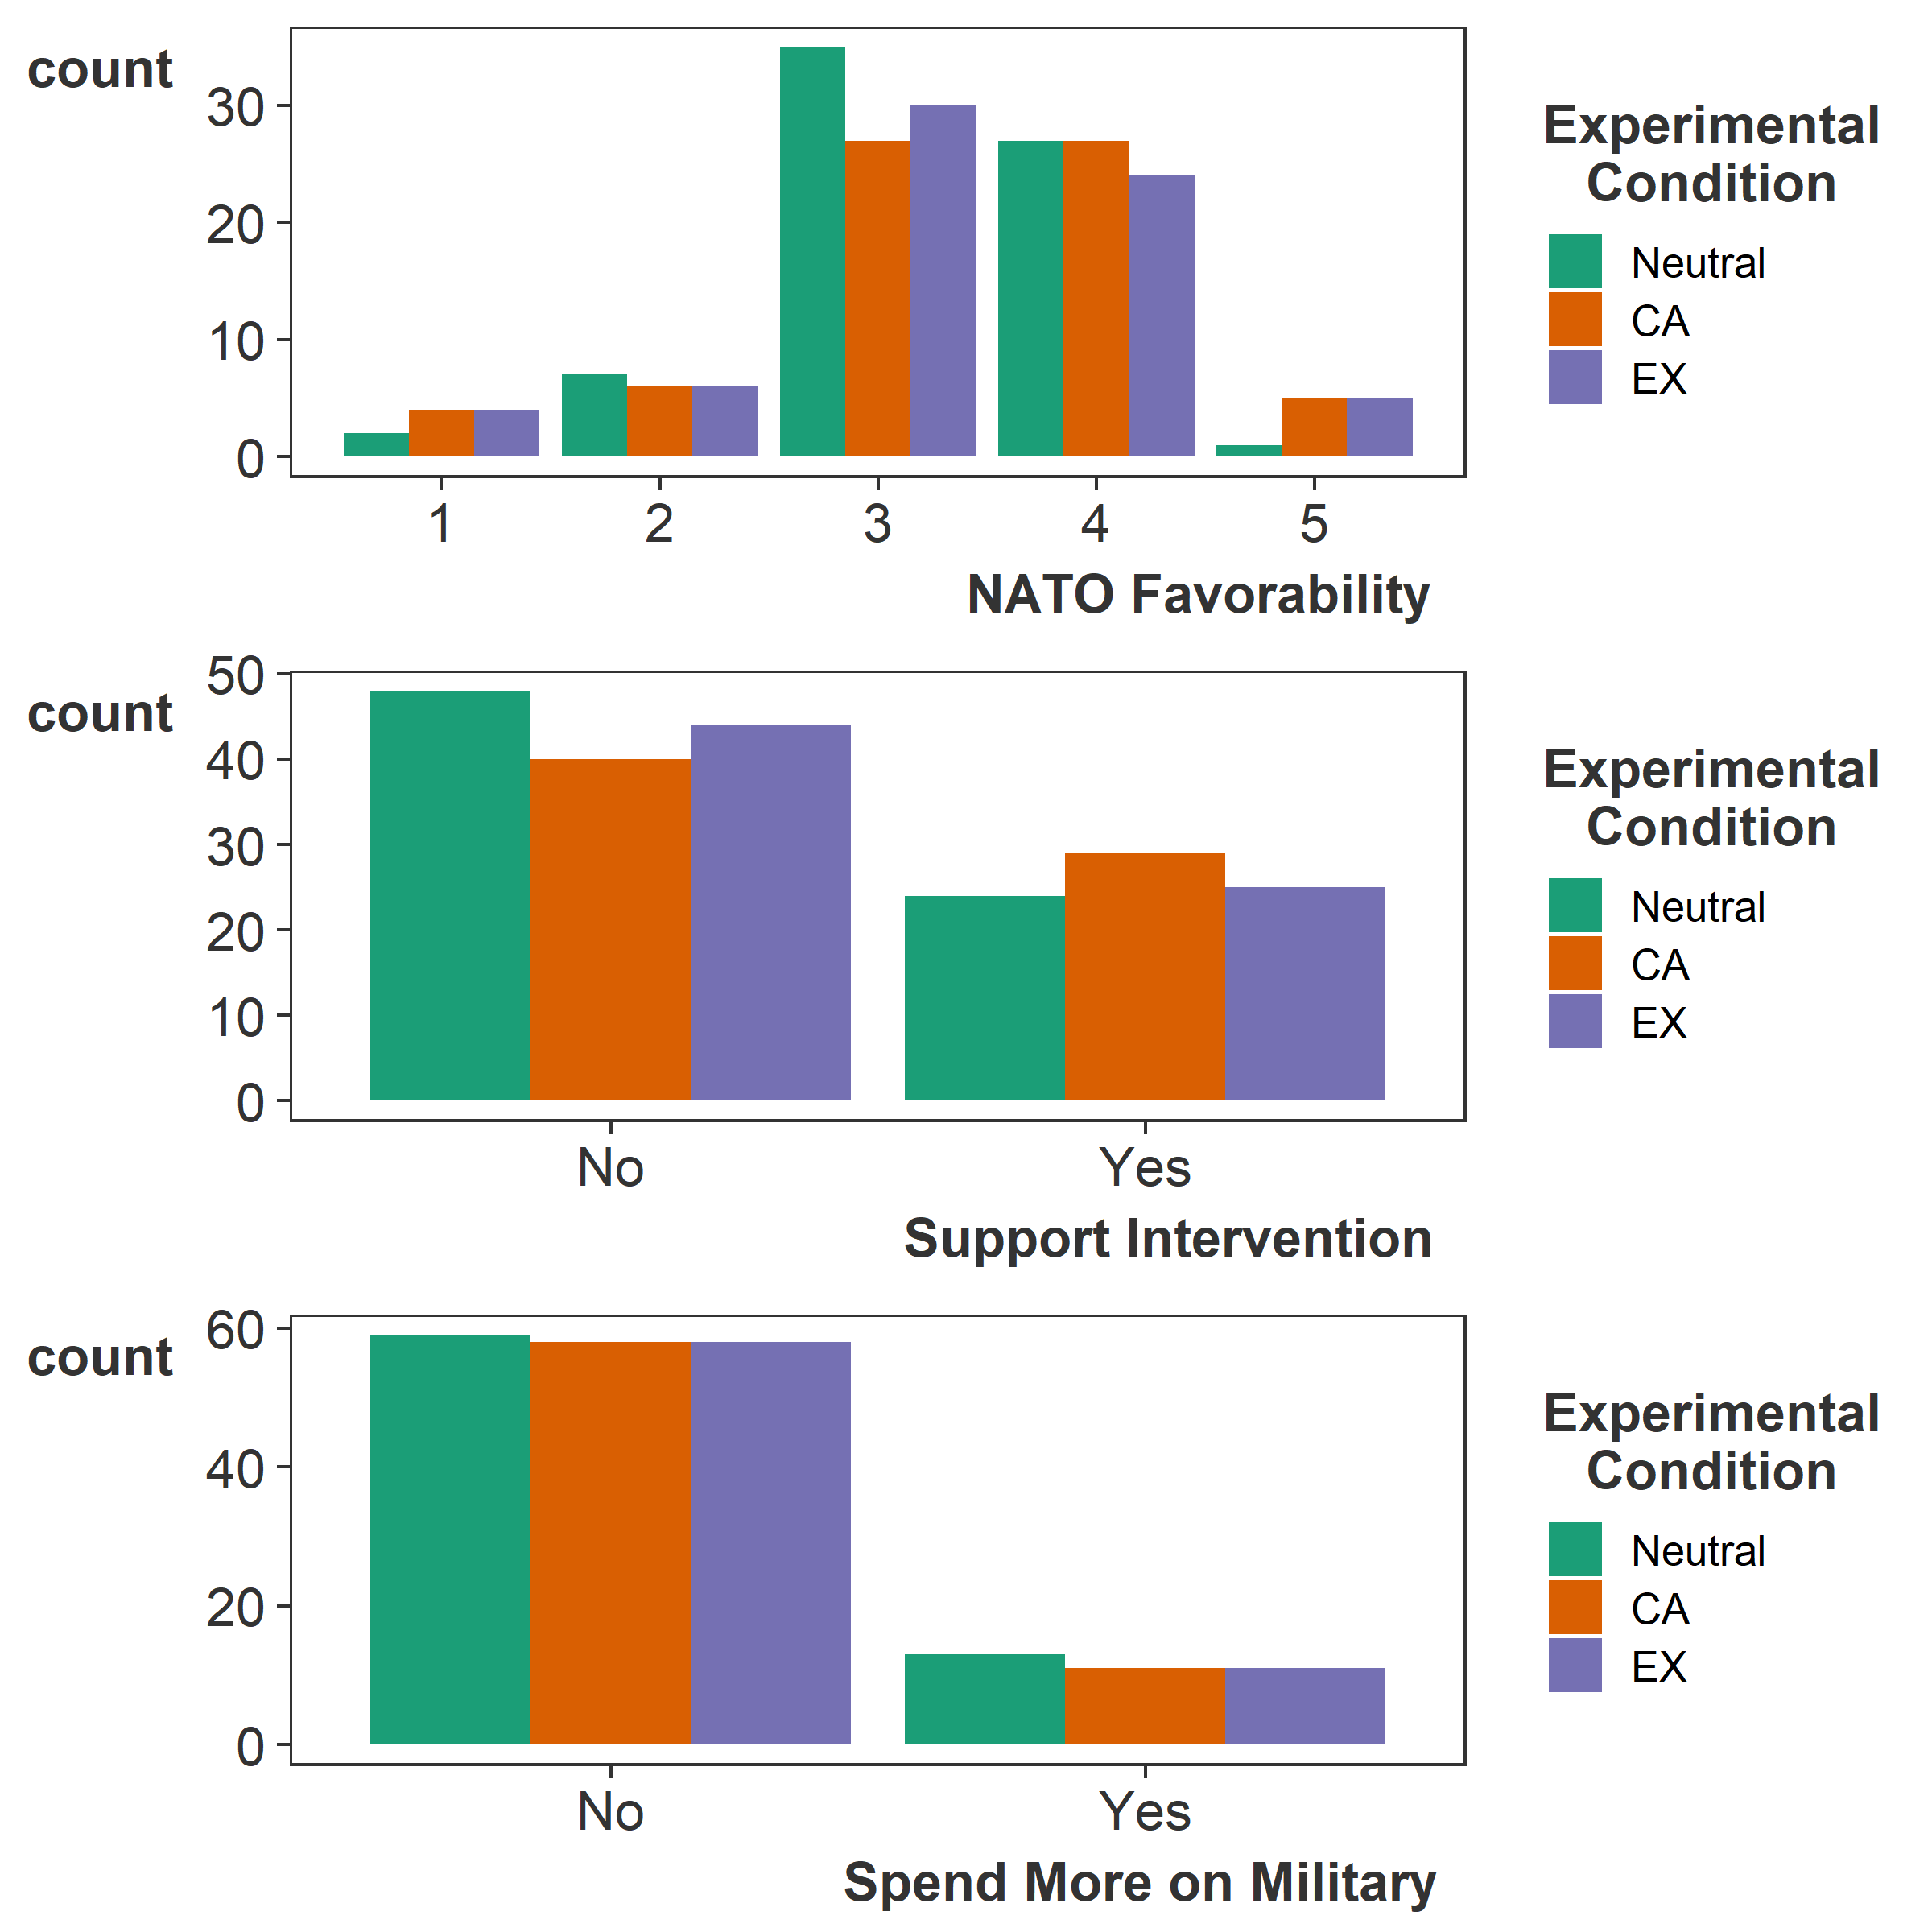
\includegraphics[height=.95\textheight]{raw-german-pres.png}
\end{figure}


\end{frame}

%-----------------------------------------------


\begin{frame}{Germany: Treatment Effects}

\begin{figure}[htbp]
	\centering
		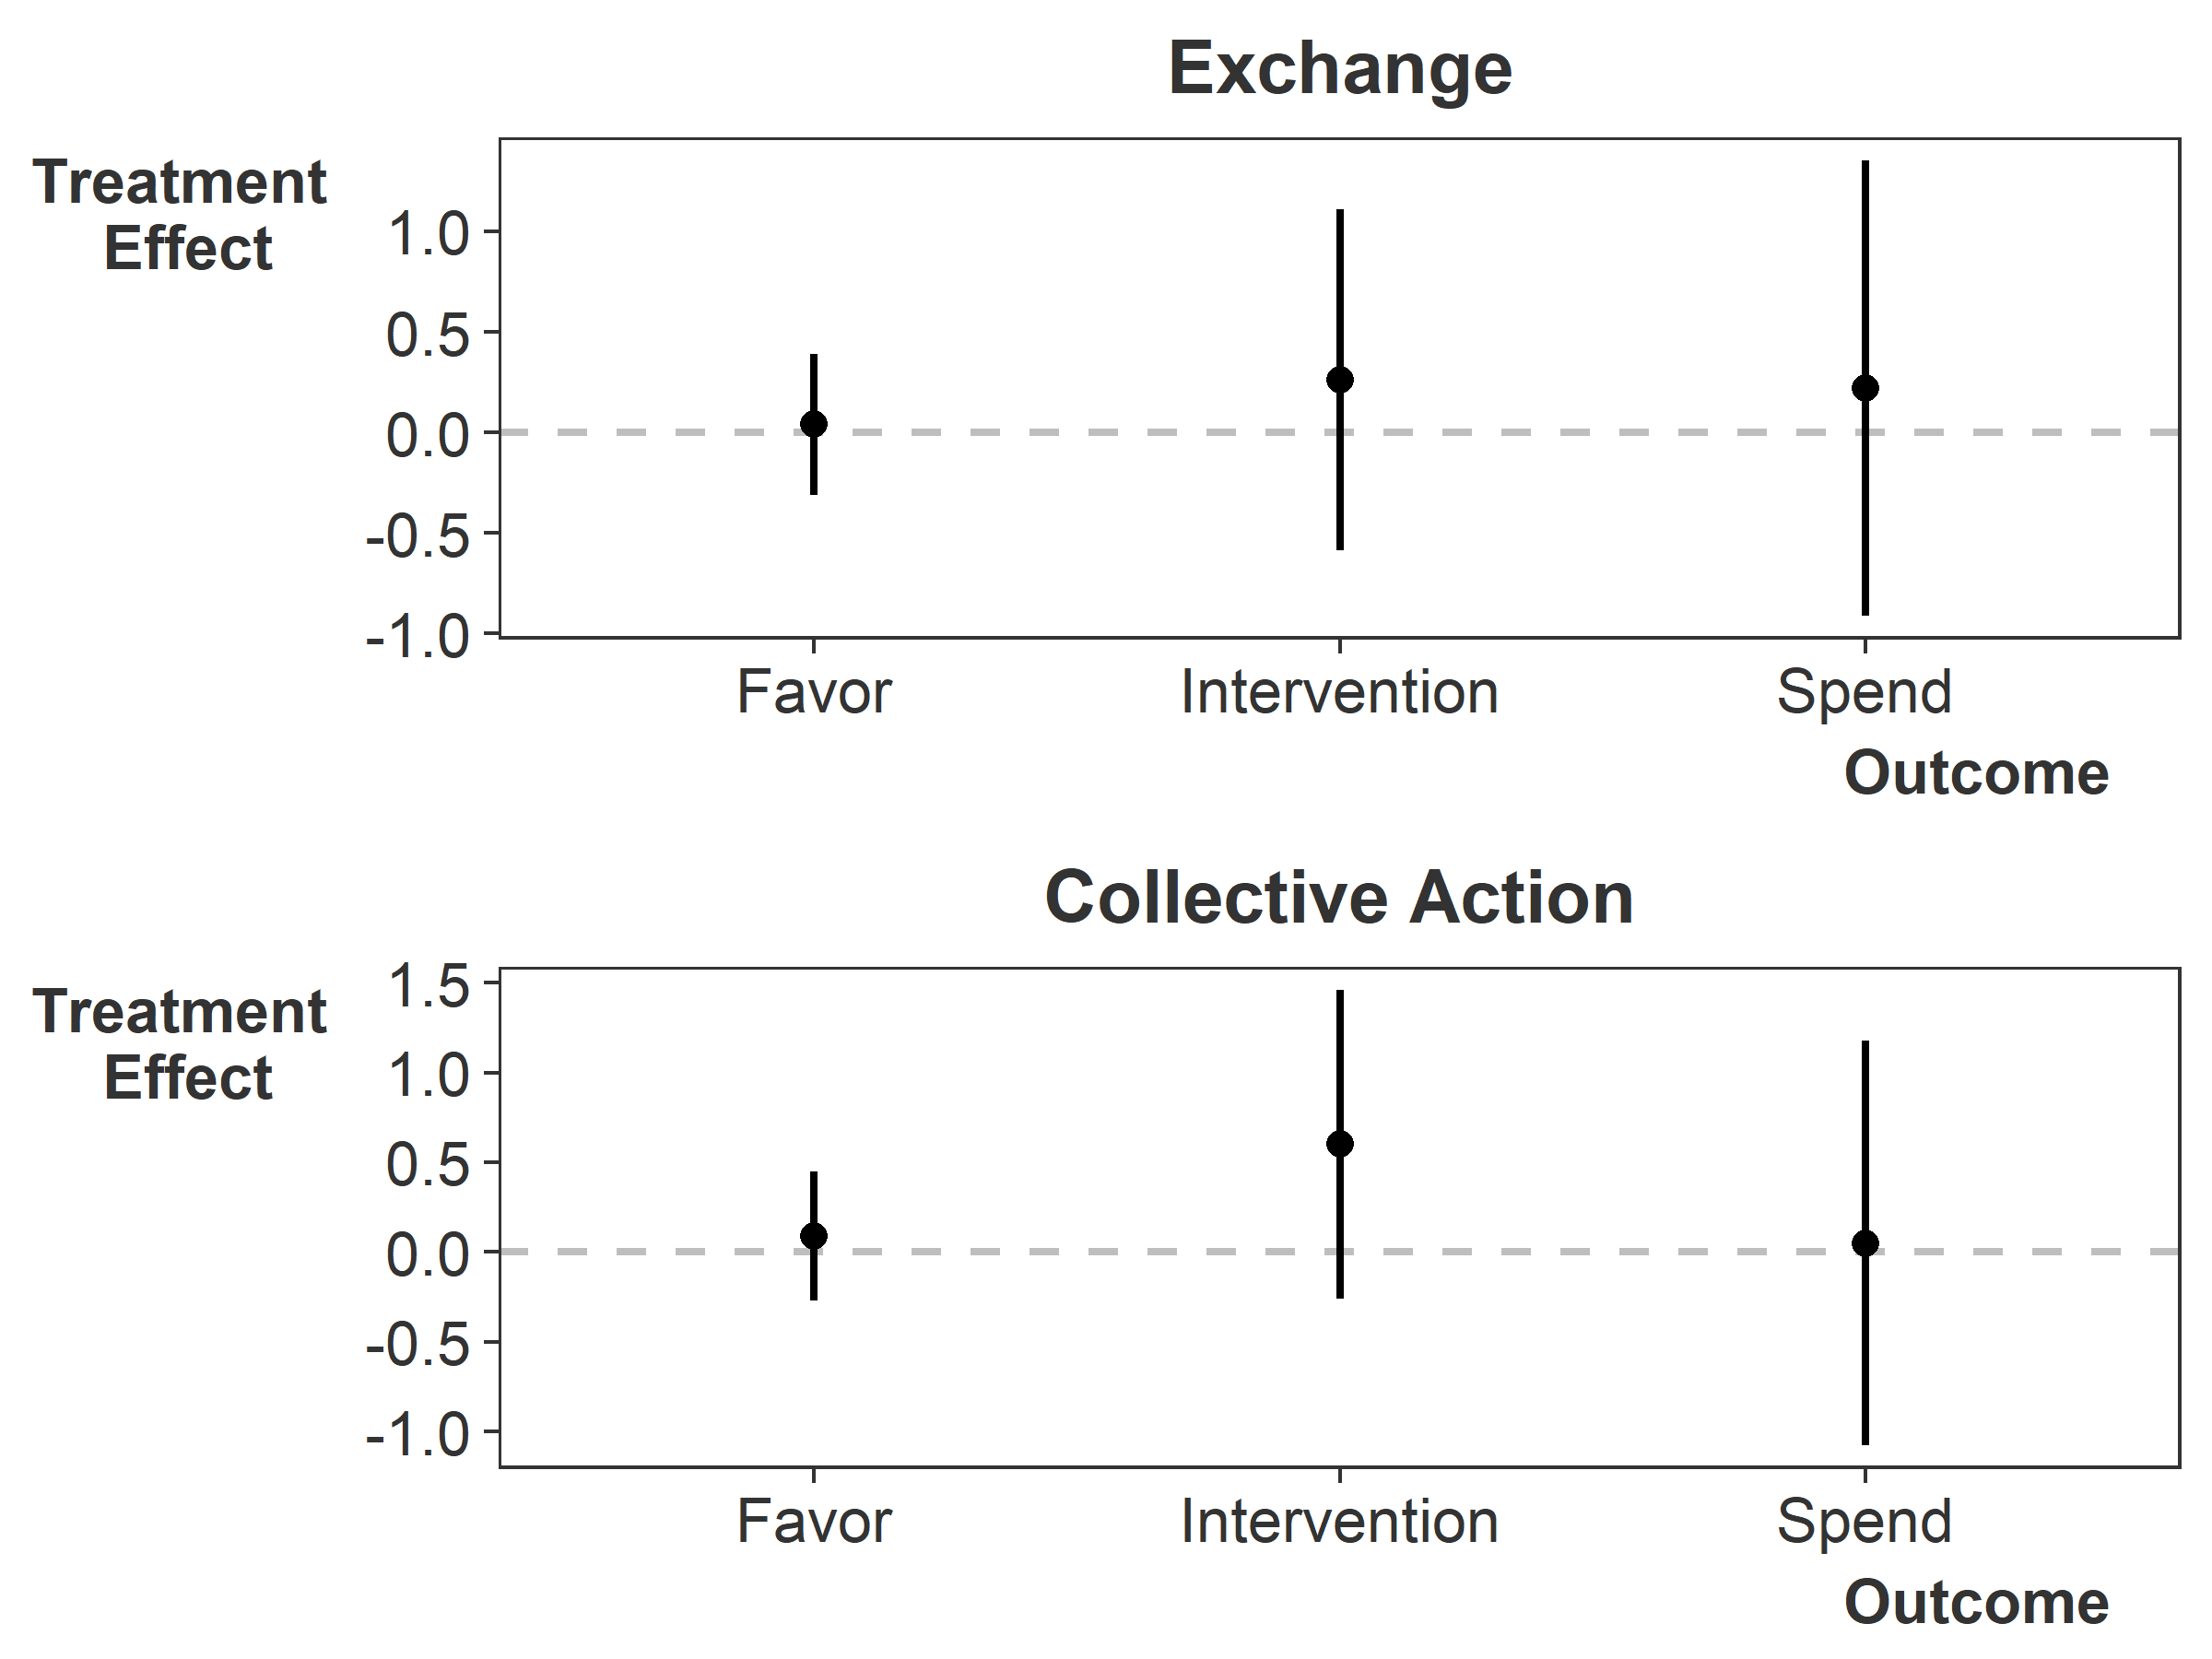
\includegraphics[width=0.95\textwidth]{ge-te-pres.png}
\end{figure}


\end{frame}


%-----------------------------------------------


\begin{frame}{Discussion}

Potential sources of weaker than expected results:

\pause
\begin{enumerate}
\item Inadequate statistical power. \pause Also hard to detect heterogeneous effects with this small sample.  
\pause 
\item Pre-treatment of collective action frames in the United States. 
\pause
\item Non-representative pre-test data.
\end{enumerate} 

\end{frame}


%------------------------------------------------

\begin{frame}{Conclusion}

This project is in the preliminary stages. I would love your thoughts on:

\pause
\begin{enumerate}
\item The argument. 
\pause
\item The experimental design. 
\end{enumerate}


\end{frame}

%-----------------------------------------------


%------------------------------------------------

\begin{frame}[standout]

Thank you! 

jkalley@virginia.edu

\end{frame}

%-----------------------------------------------

\appendix 

%-----------------------------------------------

\begin{frame}{Demographic Variables/Controls}

\begin{itemize}
\item Partisanship
\item Ideology
\item Foreign Policy Knowledge
\item National Pride 
\item Military Service
\item College Education
\item Age
\end{itemize} 

\end{frame}


%-----------------------------------------------

\begin{frame}{US Sample Concerns}

\begin{itemize}
\item Lots of Democrats
\item Above-average education
\item Above-average foreign policy knowledge. 
\end{itemize} 

\end{frame}


%-----------------------------------------------

\begin{frame}{German Sample Concerns}

\begin{itemize}
\item Lots of Greens.
\item Young (median age 27). 
\item Above-average education. 
\end{itemize} 

\end{frame}



%-----------------------------------------------


\begin{frame}{Partisanship by Group}

\begin{figure}[htbp]
	\centering
		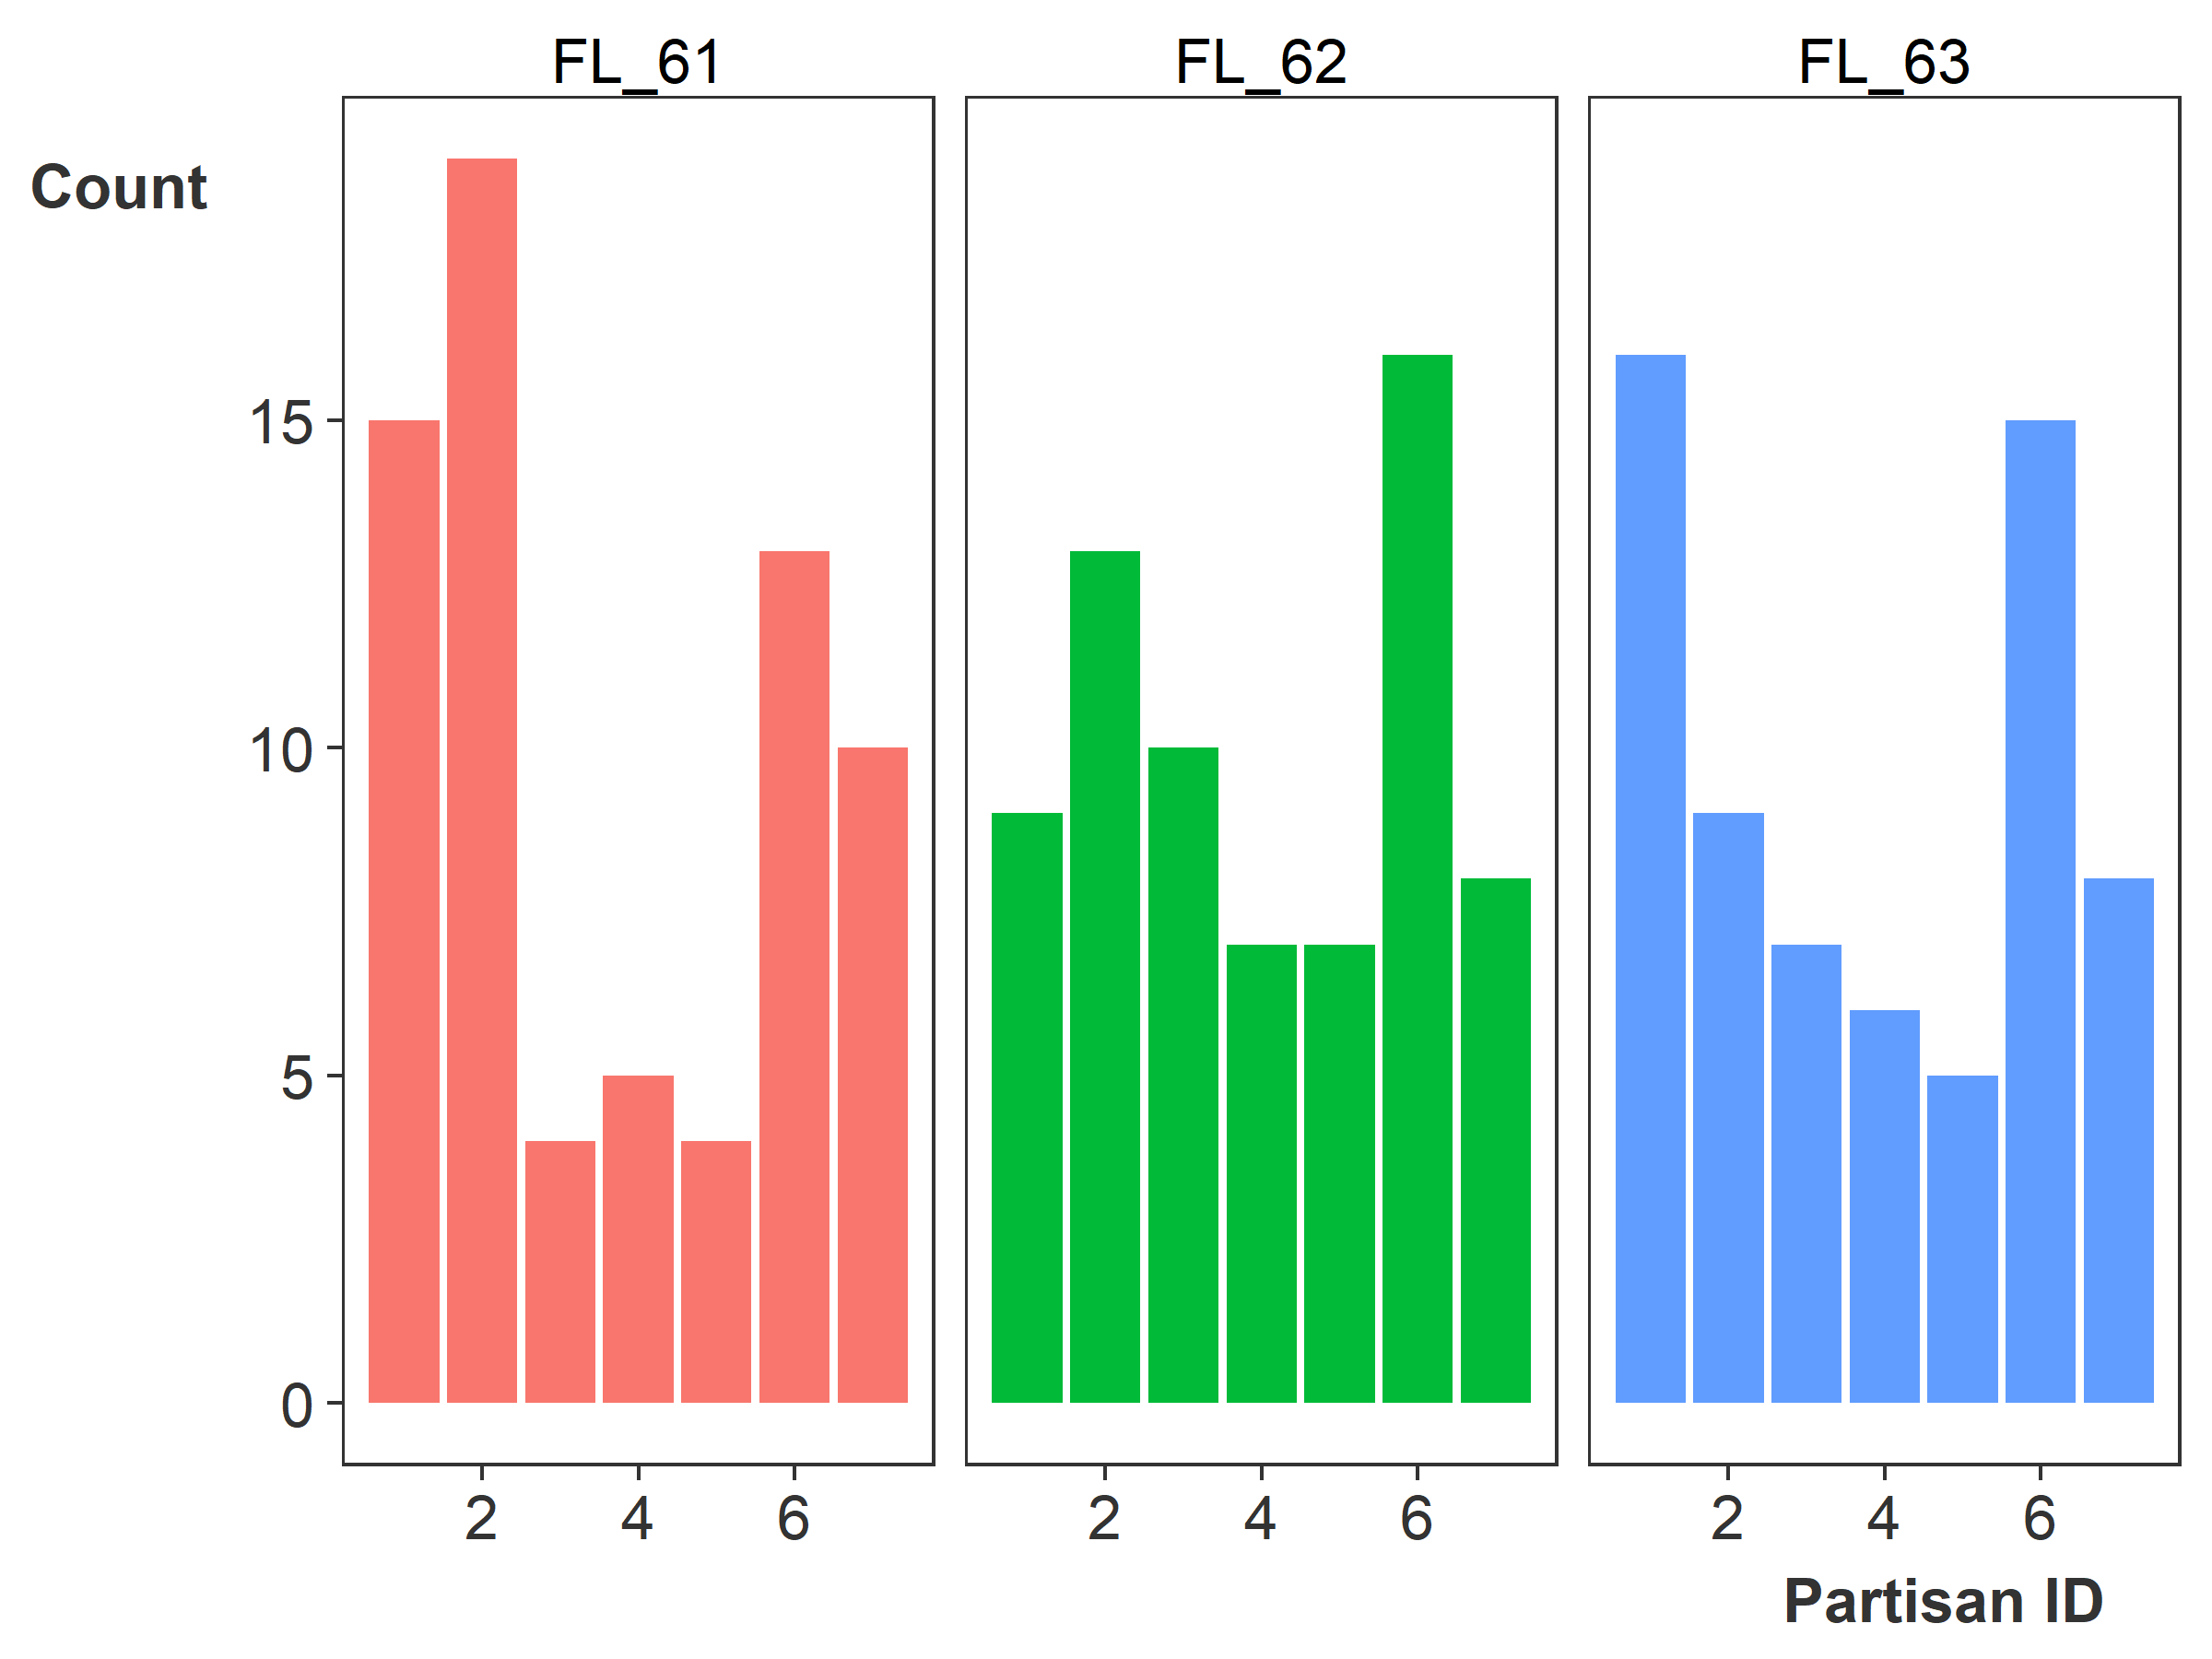
\includegraphics[width=0.95\textwidth]{partisan-group.png}
\end{figure}


\end{frame}

%-----------------------------------------------


\begin{frame}{Mechanism in Neutral Frame}

\begin{figure}[htbp]
	\centering
		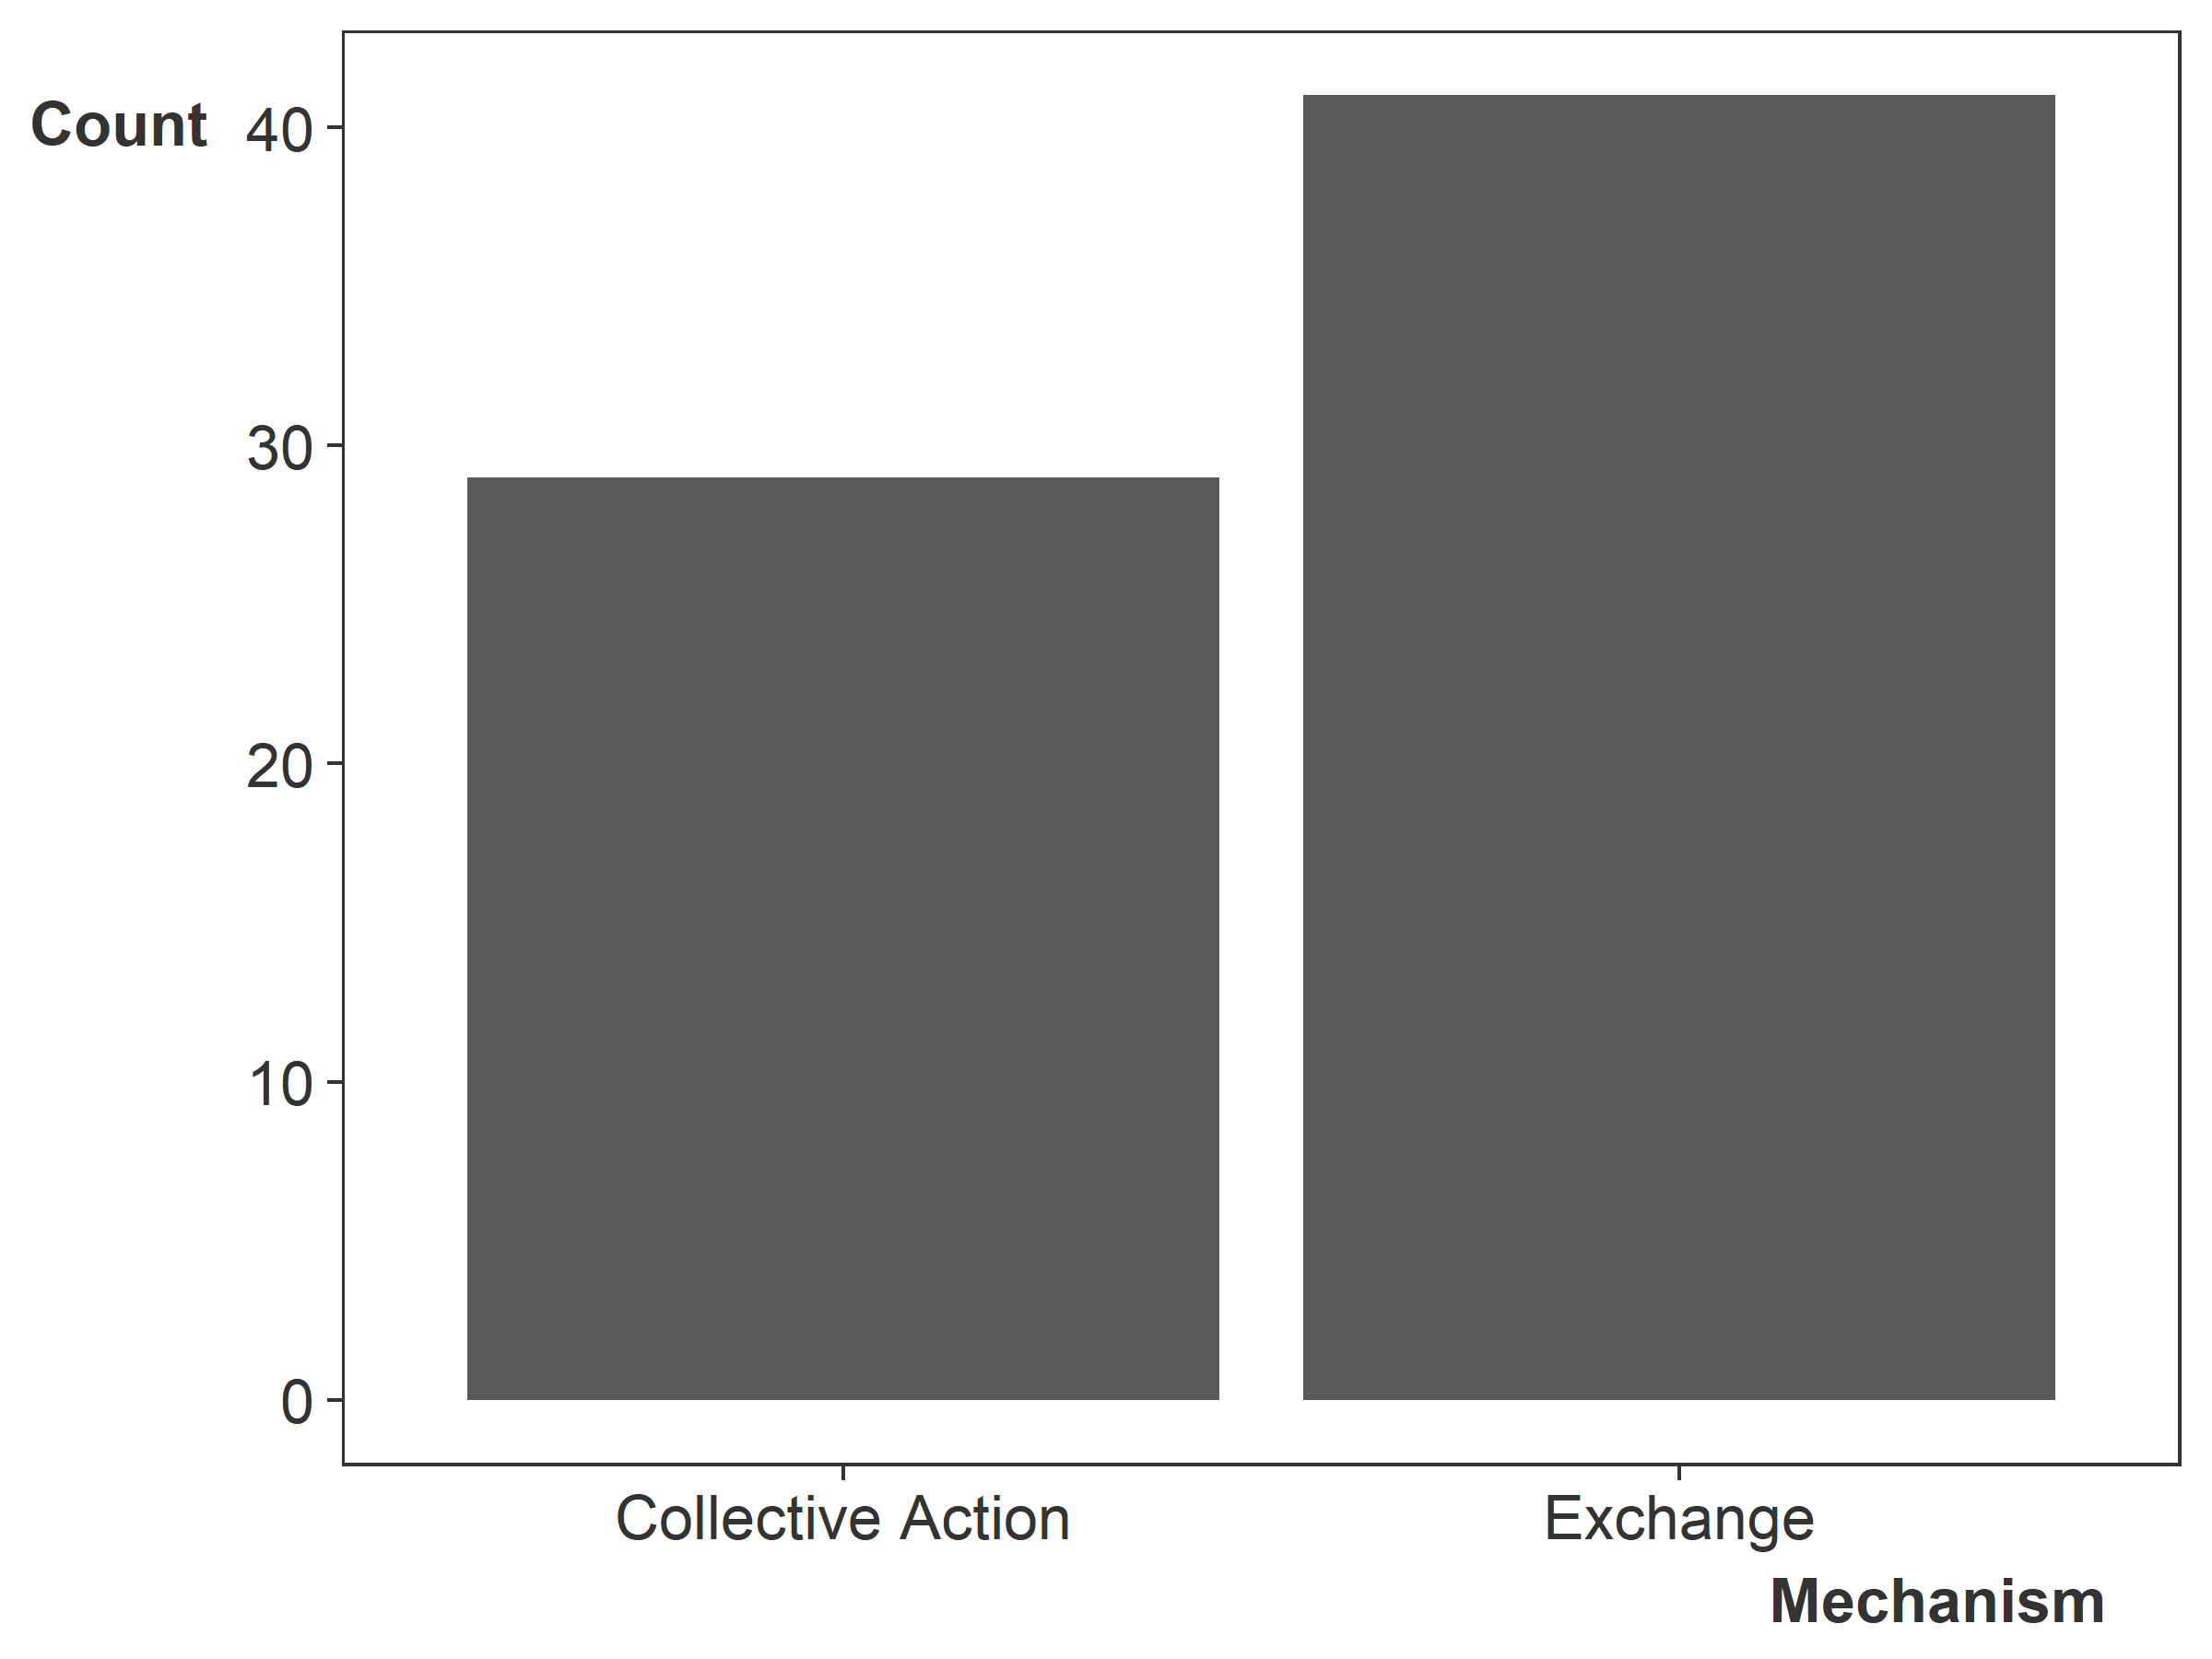
\includegraphics[width=0.95\textwidth]{neutral-mech.png}
\end{figure}


\end{frame}


%--------------------------------------------------

\begin{frame}{Map of Favorability}

\begin{figure}[htbp]
\centering
   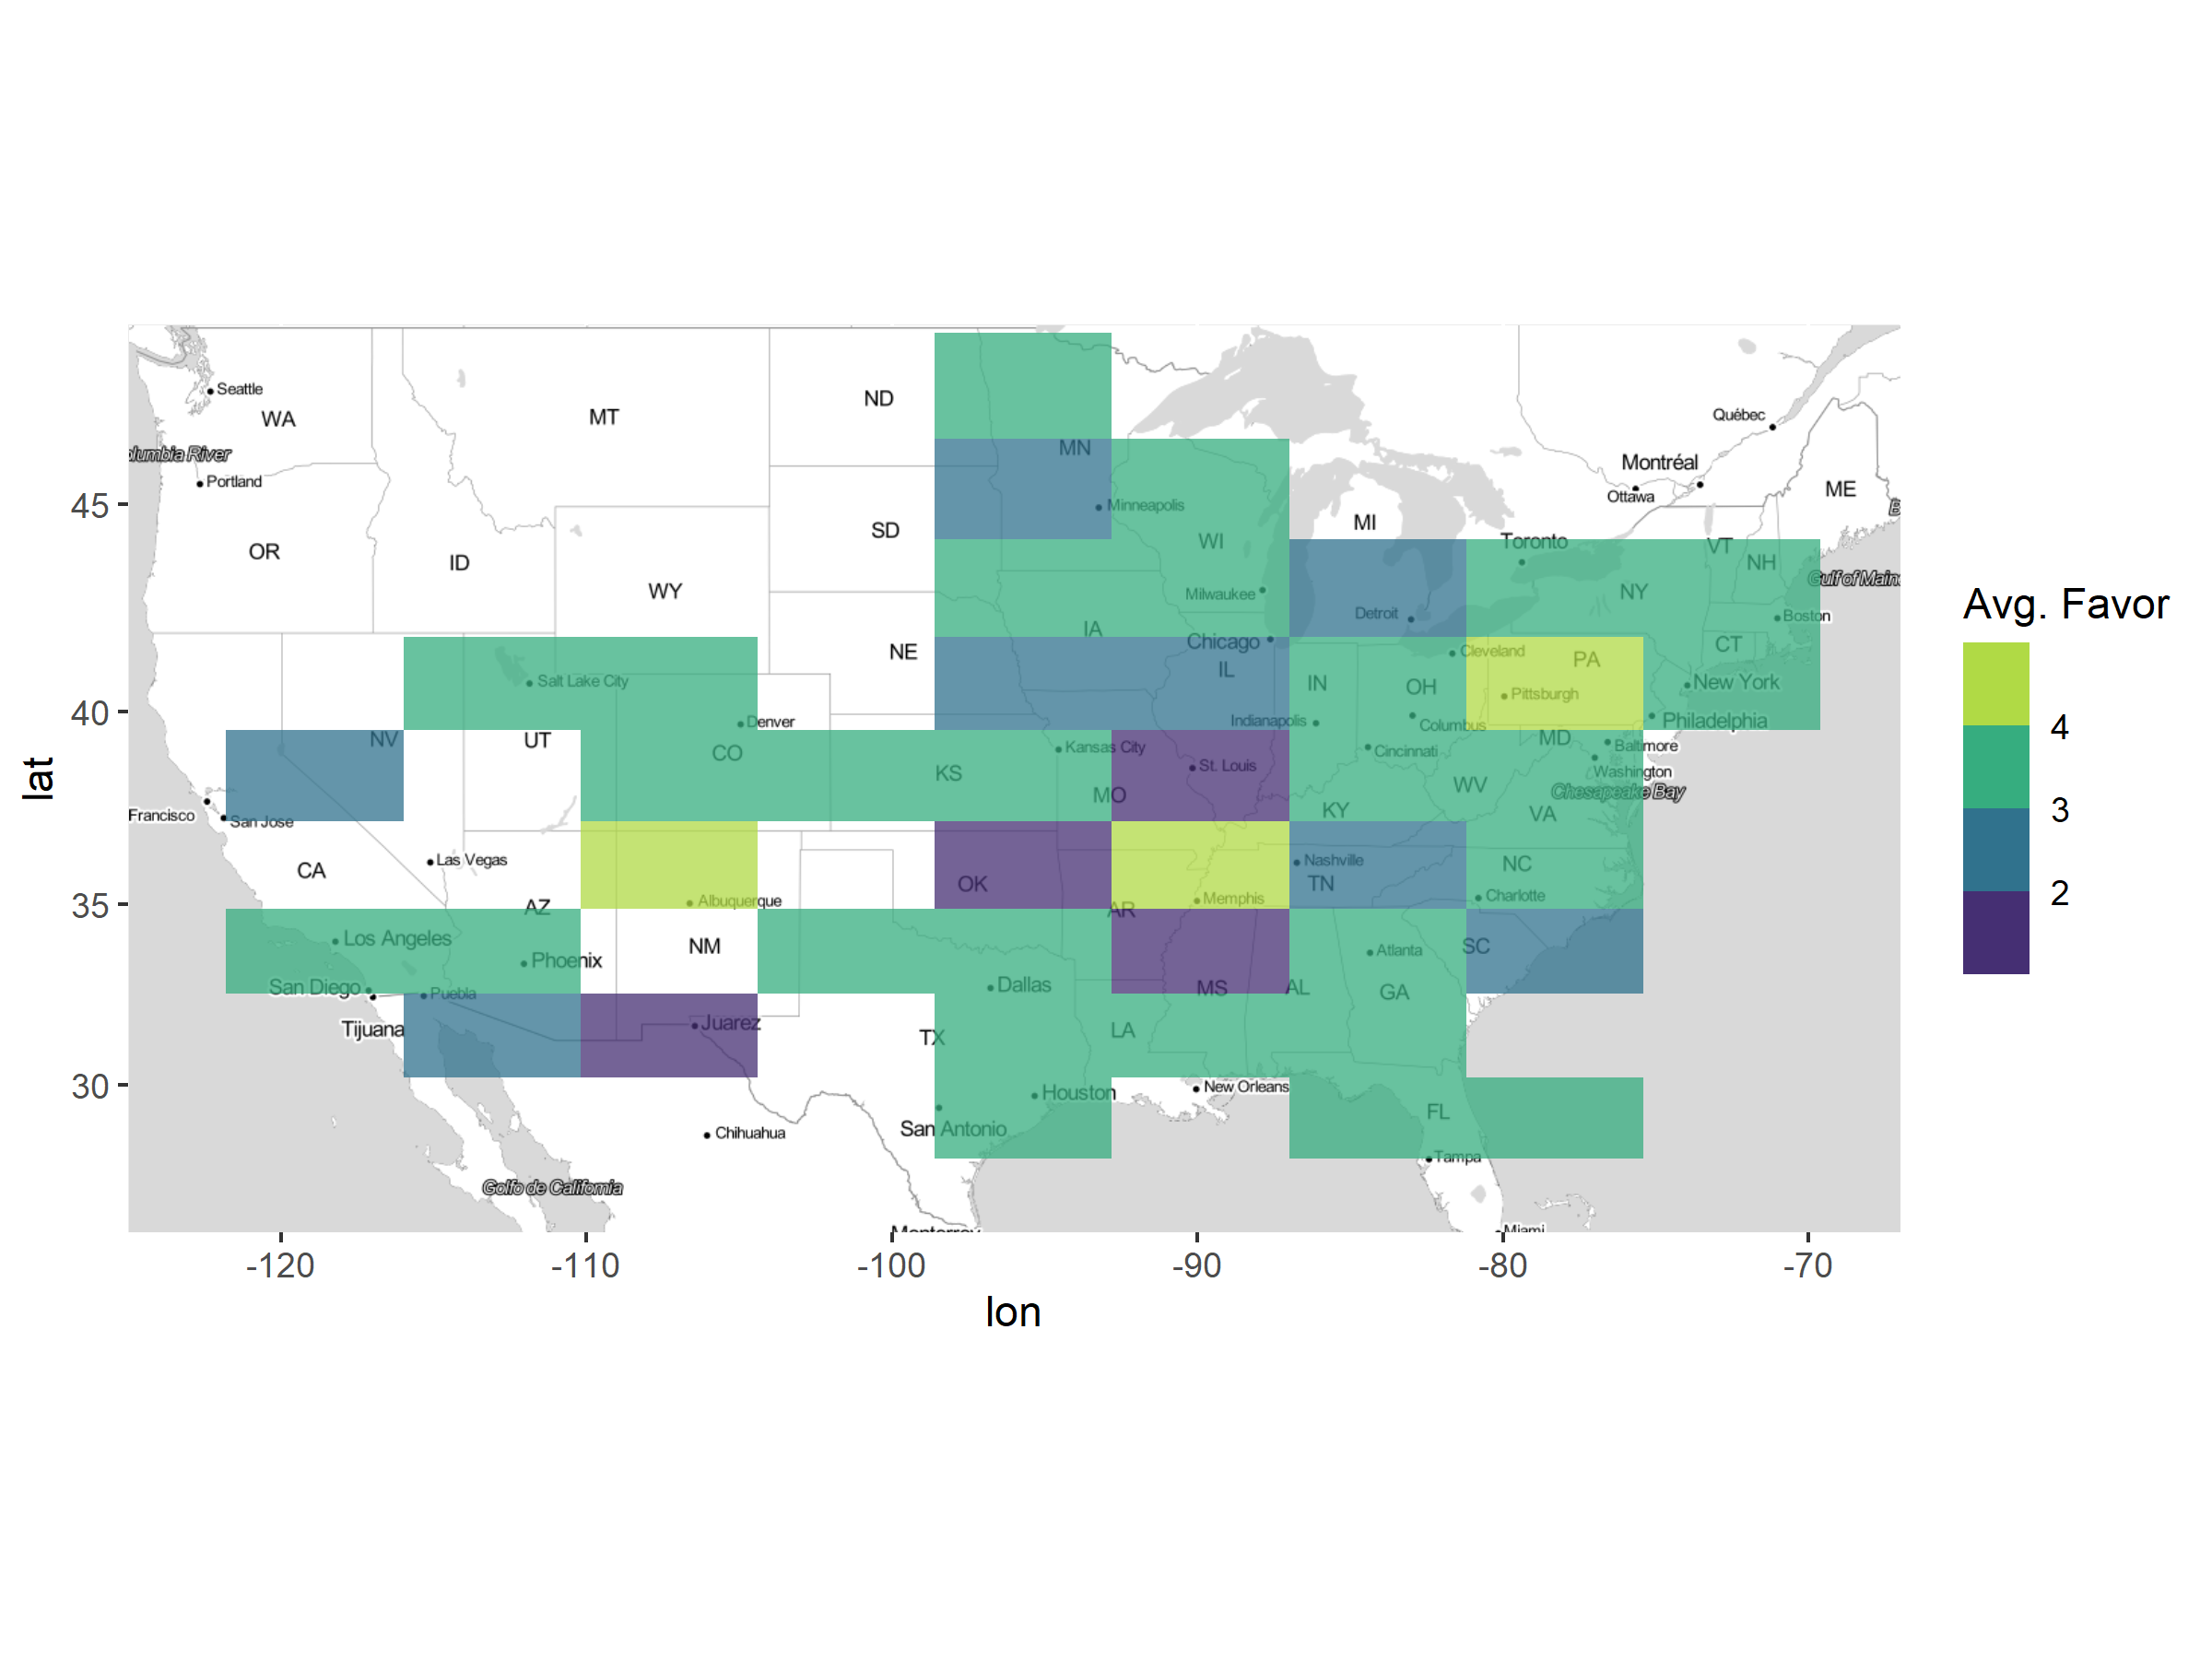
\includegraphics[width=.95\textwidth]{favor-map.png}
\end{figure}

\end{frame}

%---------------------------------------------------

\begin{frame}{Map of Support for Nonintervention} 

\begin{figure}[htbp]
\centering
   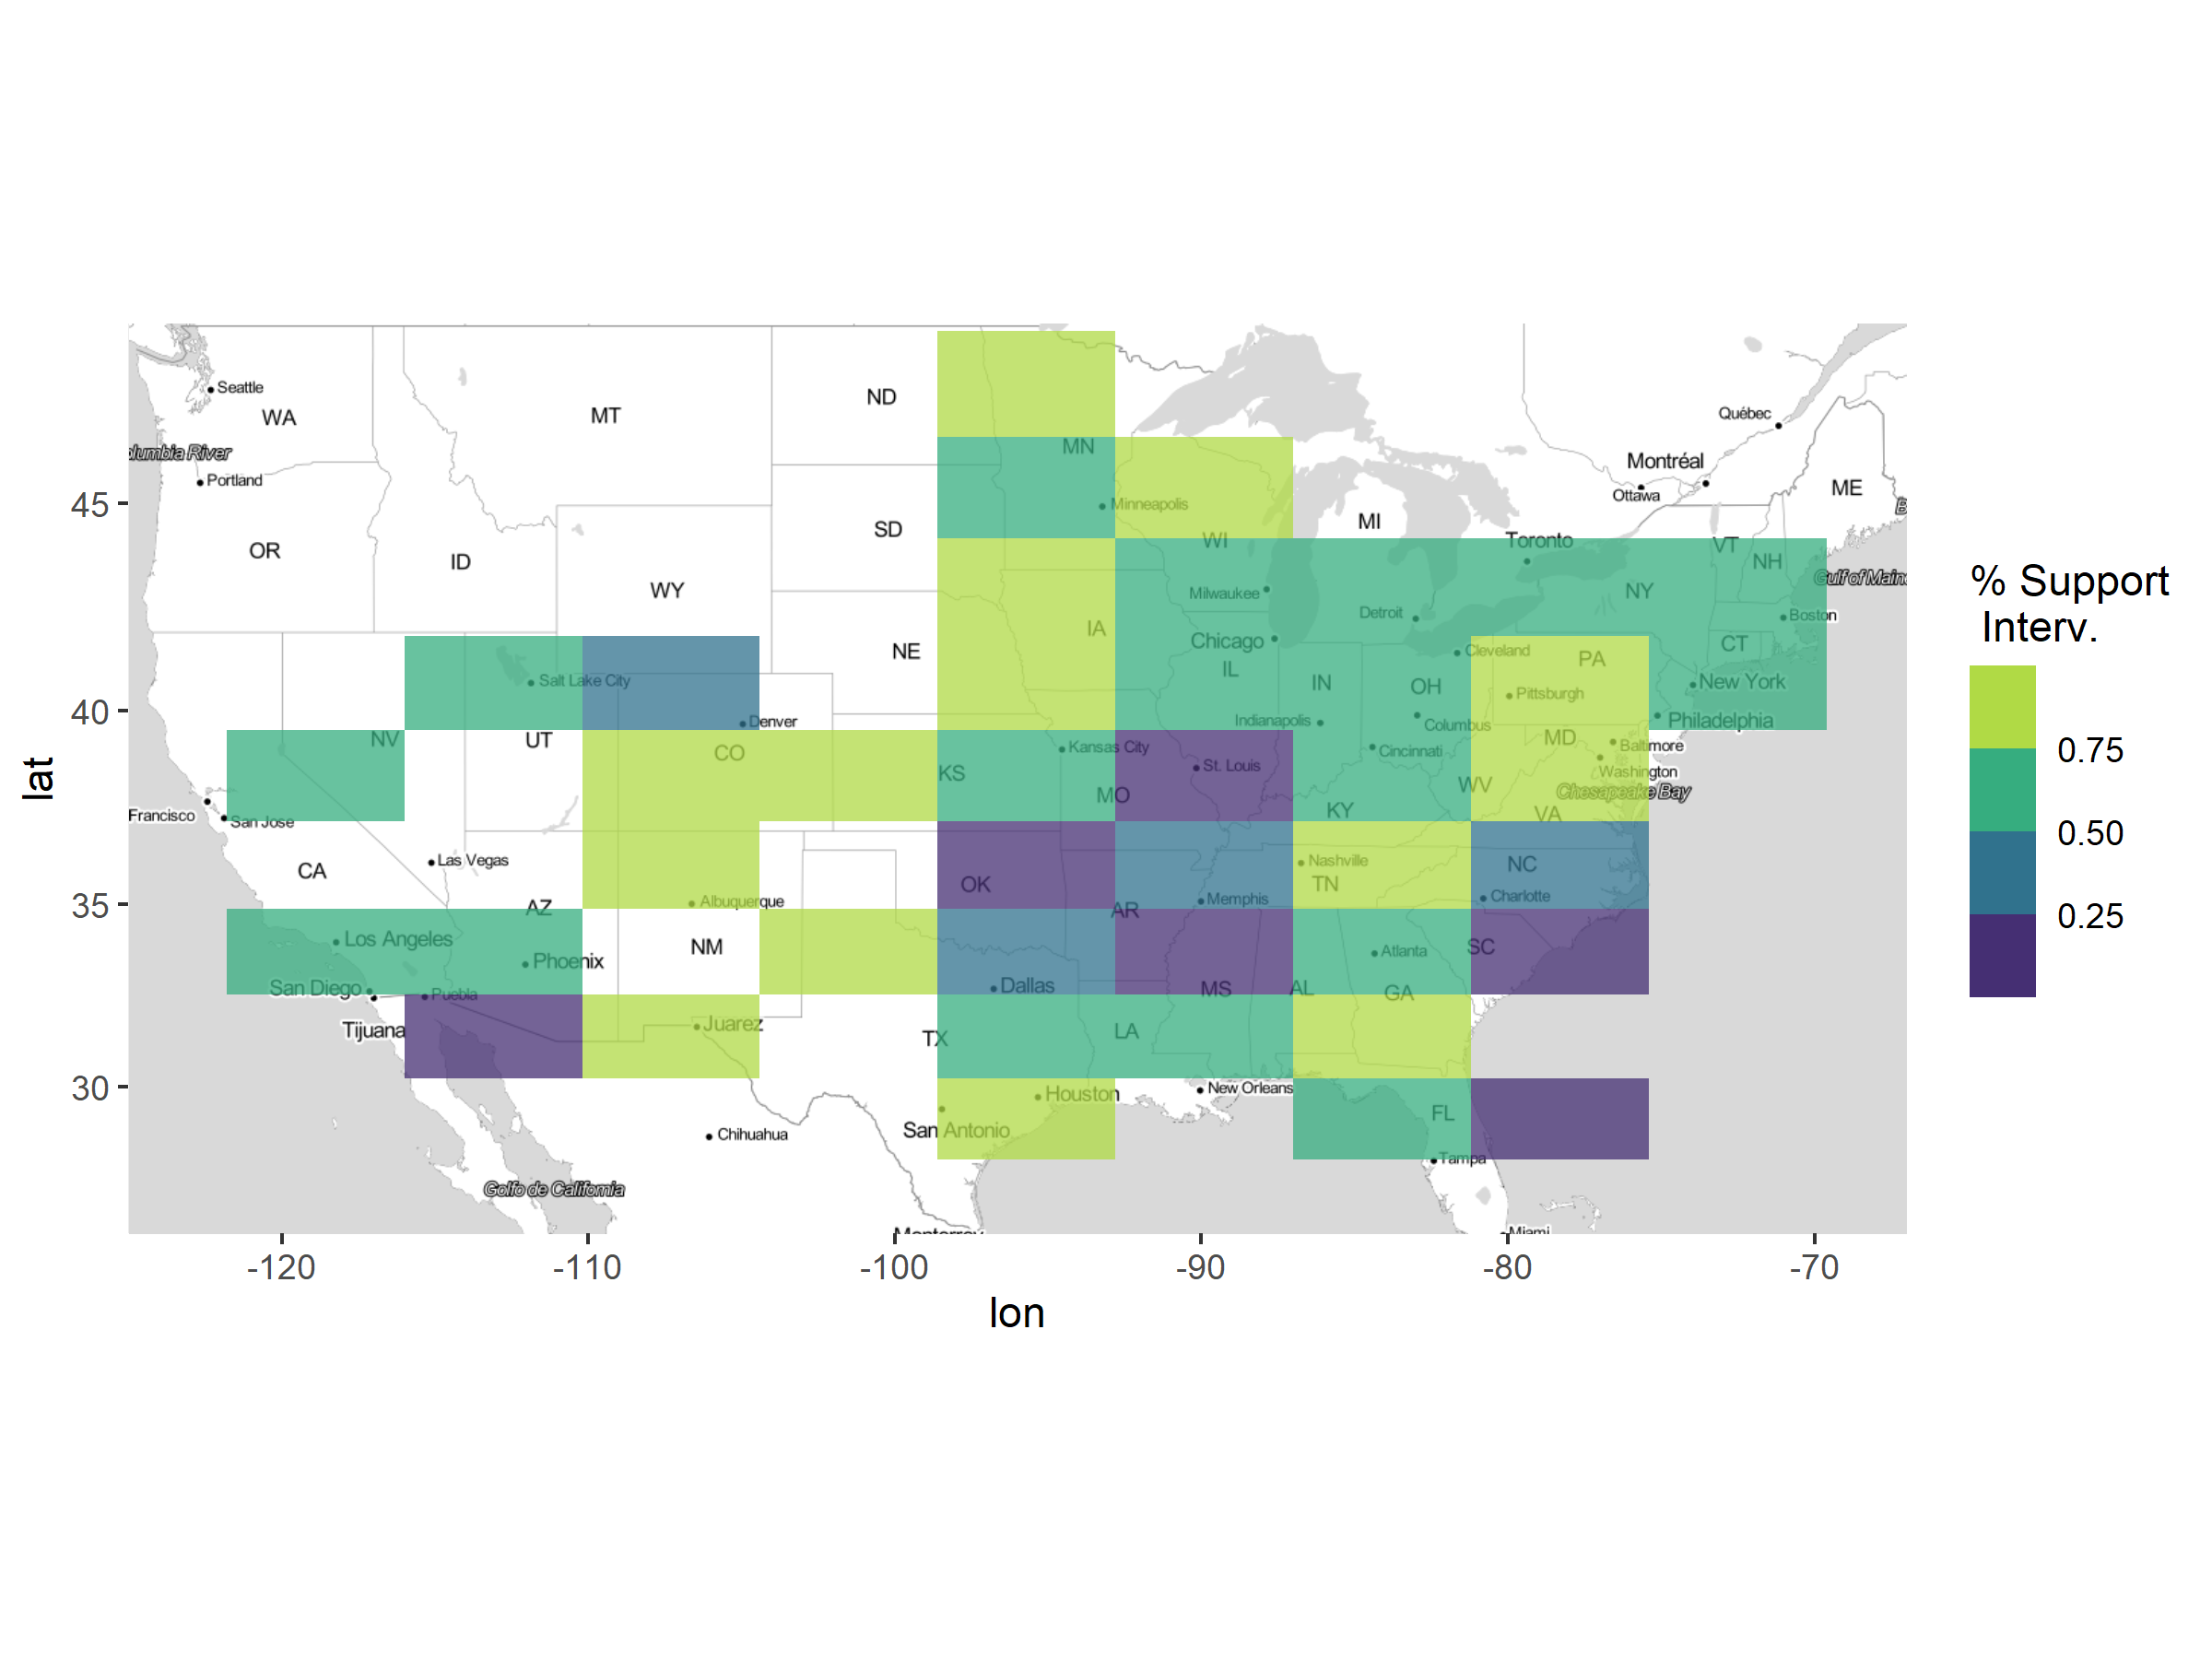
\includegraphics[width = .95\textwidth]{noforce-map.png}
\end{figure}

\end{frame}

%---------------------------------------------------



%----------------------------------------------------------------------------------------

\end{document}
